\documentclass[11pt,english]{article}
\usepackage{ae,aecompl}
\usepackage{helvet}
\usepackage[T1]{fontenc}
\usepackage[square,numbers]{natbib} 
\usepackage{amssymb,amsmath,amsthm}
\usepackage[nolists]{endfloat}
\usepackage{graphicx}
\usepackage[pdfborder={0 0 0}]{hyperref}
\usepackage{chngpage}
\usepackage{pdflscape}
\usepackage{epstopdf}
\usepackage{fullpage}
\usepackage{setspace}
\usepackage{booktabs}
\usepackage[small,compact]{titlesec}
\usepackage{rotate}
\usepackage{caption}
\usepackage{subcaption}


\usepackage{hyperref}
%\usepackage[hidelinks]{hyperref}
\usepackage{xr-hyper}
\usepackage{xr}
\externaldocument{PrimaryLightingFuel_APPENDIX}

\newcommand{\noun}[1]{\textsc{#1}}
\newcommand{\citetapos}[1]{\citeauthor{#1}'s \citeyearpar{#1}}
\providecommand{\tabularnewline}{\\}

\theoremstyle{plain} \newtheorem{claim}{Claim}
\theoremstyle{plain} \newtheorem{prop}{Proposition}
\theoremstyle{plain} \newtheorem{hypo}{Hypothesis}

%\bibpunct[: ]{(}{)}{;}{a}{,}{,}


\begin{document}

\title{Lock-in for lighting: The puzzle of continued kerosene use among electrified households in six Indian states\footnote{Fully documented data and code are available on Harvard Dataverse at \url{https://doi.org/10.7910/DVN/PVWSOY}. We thank Micha\"{e}l Aklin, Brian Blankenship, Elisha George, and Sonakshi Saluja for their valuable comments on the manuscript.}}

\author{Xiaoxue Hou\\Johns Hopkins SAIS \and Johannes Urpelainen\footnote{Corresponding author. Address: Rome Building, 4th Floor. 1619 Massachusetts Avenue, NW. Washington, DC 20036, USA. Tel: +1-734-757-0161. Email: JohannesU@jhu.edu.}\\Johns Hopkins SAIS}
\maketitle


\begin{abstract}

Electricity is the most commonly used form of energy for artificial lighting in modern society. Despite a rapid growth in the rate of electrification, 9\% of electrified Indian households in our six sampled states continued to use kerosene as their primary lighting fuel in 2018. This appears as a puzzle considering the benefits of electric lights. Using a panel survey of rural households in six states in India, we examine why some grid-connected households primarily used kerosene lamps for illumination. We use a logistic regression model to test our hypothesis regarding the relationship between primary lighting choices and electricity quality. The results show that household primary lighting choices are correlated with nighttime duration of electricity service, daytime duration of electricity service, and the number of days without any electricity connection, at the 99\% confidence level. Among these three factors, nighttime duration of electricity service has the greatest impact. To further promote the use of electric lights, intensive schemes to improve electricity quality are needed.

\end{abstract}

\textbf{Keywords}: Rural electricity; Energy access; Energy poverty
\clearpage
\doublespacing

\section{Introduction}

Modern energy access is an important prerequisite for societal development. Electric lighting, in particular, benefits households by improving health outcomes and children$'$s study environment, while the use of kerosene lamps causes potential accidents and health risks, such as eye and respiratory diseases \citep{Vandewalleetal2013, BarronTorero2017, Bruceetal2000, Worldbank2008}. Still, a considerable number of households around the globe continue to use kerosene for lighting, even among already electrified groups \citep{Lametal2016}. Considering the benefits of replacing kerosene lamps with electric lights, it is a puzzle as to why electrified households continue to use kerosene as their primary lighting option.

Recognizing the importance of electrification for rural development, the Indian government strengthened its commitment to electricity reform by enacting the Electricity Act in 2003 and promising $``$Power for All$"$ by 2012. To achieve the first stage of supplying power to all villages, India launched the Rajiv Gandhi Grameen Vidyutikaran Yojana (RGGVY) Scheme in 2005. Despite India$'$s laudable progress in achieving a 92\% village electrification rate, 311 million people, mostly living in rural regions, still had no access to electricity in 2012 \citep{Banerjeeetal2014}. Hence, kerosene lamps were used by a large portion of people in India. Based on Lam et al. (2016) \citep{Lametal2016}, in 2011, 380 million people in India relied on kerosene lamps for primary lighting. The issue had persisted and 45 million households did not have electricity access used in 2017 \citep{PalitBandyopadhyay2017}. In Assam, for example, 62\% of households used kerosene for lighting \citep{Barmanetal2017}. With the objective of electrifying all remaining households, the Government of India launched the Pradhan Mantri Sahaj Bijli Har Ghar Yojana (the Saubhagya Scheme) in 2017, which offered free electricity connections and distributed free LED lights to households that were below the poverty line. As a result of these efforts, the percentage of households using kerosene as the primary fuel has declined significantly after the enactment of the Saubhagya Scheme.

Indian people, however, have a long history of relying on kerosene for lighting purposes. Instead of giving up the fuel, people tend to store it for use during electricity service disruptions, partially due to the long-lasting kerosene subsidies. In Dharampur, kerosene usage surged following the disruption of the electricity supply network due to heavy rainfall, highlighting the crucial role it plays in the daily life of rural Indians \citep{Mehta2019}. In fact, some electrified households even choose to use it as their primary lighting source. Based on our analysis, 9\% of grid-connected Indian households relied on kerosene as their primary lighting fuel in 2018. To achieve the government$'$s $``$Power for All$"$ target and fully realize the benefits of electrification, it is very important to understand the motivations behind continued kerosene use.

We aim to answer the following question: $``$Why do Indian households continue to use kerosene despite having access to electric lighting?$"$ by studying grid-connected households$'$ preferences in six Indian states: Madhya Pradesh, Bihar, Jharkhand, Uttar Pradesh, Odisha, and West Bengal. Our analysis uses the most recent survey data on Indian household energy access, Access to Clean Cooking Energy and Electricity - Survey of States (ACCESS) \citep{Aklinetal12016, Jainetal2018}. It contains detailed questions on household energy situations and their patterns of usage. It provides data from two rounds of surveys conducted in 2015 and 2018. The survey offers a large-N panel dataset with the same set of households investigated in both rounds. For the purpose of our study, we analyze the lighting preferences of 4,924 households that had grid electricity in both rounds. To determine the influence of insufficient and interrupted power on households$'$ choices of primary lighting source, we use a logistic regression to analyze the relationship between households$'$ primary lighting choices and the quality of electricity service. Household electricity quality is characterized by adequacy and reliability. In the survey data, adequacy is quantified by the daily duration of electricity connection and reliability by the outage days (defined as the number of days without any electricity connection). We also include confounders and pre-treatment covariates to increase precision and reduce bias in the models. To represent the electricity supply situation among the population, we use descriptive statistics to show household satisfaction on four aspects of electricity service including safety, reliability, adequacy, and affordability. The results from our analysis suggest that poor electricity quality, characterized by short durations of electricity connection and frequent electricity outage days, is possibly hindering households transitioning from kerosene lamps to electric lights.


We find that the proportion of electrified households that used electricity as their primary lighting source increased from 66\% in 2015 to 91\% in 2018. Poor electricity quality is still a major concern among Indian households. Nighttime duration of electricity service has a greater effect on households$'$ primary lighting fuel choice than daytime duration. Increasing nighttime duration of electricity service by one hour, on average, increases the probability of adopting electricity as the primary lighting source by 4.05 percentage points (95\% confidence interval (CI): 3.6-4.5 percentage points). A one-hour increase in daytime service will lead to 1.50 percentage points (95\% CI: 1.33-1.66 percentage points) increase, smaller than the effect of night hours. The number of electricity outage days also shows a significant influence on the choice of primary lighting fuel at the 99\% confidence level. A one-day increase in monthly outage days results in a 0.31 percentage point (95\% CI: 0.18-0.44 percentage points lower) decrease in the probability of adopting electricity as the primary lighting fuel, on average. Hence, we find that electricity quality is an important factor in determining a rural household$’$s choice of primary lighting fuel in the six energy-deprived states in India. In order for Indian households to transition towards the use of cleaner lighting options, the quality of the electricity supply must be improved.


\section{Kerosene Fuel and Electric Lighting}

The awareness campaign of clean lighting options has spanned decades, encouraging rural households to use less harmful and more efficient lighting sources. Nonetheless, 9\% of electrified households in our survey still chose kerosene as their primary lighting fuel in 2018. The continued use of kerosene lights prevents the rural population from availing the public health benefits and safety of modern lights \citep{BarronTorero2017}.

Studies have shown that kerosene, no matter if used as lighting or cooking fuel, causes indoor air pollution that leads to serious health risks \citep{Lametal2012}. The particles and poisonous gases generated from kerosene fumes cause eye and respiratory diseases \citep{Lametal2012, Appleetal2010}. In addition, kerosene wick lanterns and candles, which are used in poorly ventilated indoor spaces, can give rise to safety risks associated with unattended fires \citep{BringulaBalahadia2019}. Furthermore, both safety and health risks are exacerbated by the long duration of human exposure to the kerosene lamps. For example, when children sit by the faint and flickering light for hours while studying, the pungent odor of open wick kerosene lamps makes them particularly vulnerable to these risks.

In addition, using kerosene for lighting is also inefficient. Dutt and Mills (1994) \citep{DuttMills1994} and Mahapatra et al. (2009) \citep{Mahapatraetal2009} both discussed the poor quality of kerosene-based lighting. The illumination from kerosene lamps is far less than that provided by the modern electric lighting while most energy is wasted in the form of heat \citep{Mills2005}. The poor light output along with the massive energy usage manifests the inefficiency of this type of lighting. Without the market distortions caused by the massive kerosene subsidies, the use of kerosene lamps is not economically appealing either. According to Mahapatra et al. (2009) \citep{Mahapatraetal2009}, if we consider the open market price for kerosene, the cost of useful energy for a kerosene wick lamp is the highest among different lighting sources.

On the other hand, electricity from grid access provides people with a highly efficient and less polluting option for indoor lighting. Since lighting is one of the basic needs and the dominant purpose of households using electricity \citep{Worldbank2008, Bernard2012}, electric lights are expected to be promptly used as the primary lighting source as soon as people get grid access. However, connection to the grid does not directly translate to a shift from kerosene lamps to a full reliance on electric lighting. According to Cheng and Urpelainen (2014) \citep{ChengUrpelainen2014}, in 2010, only around 25\% of rural Indian households relied exclusively on electricity for lighting purposes. More than half the population is trapped in a phenomenon called $``$fuel stacking$"$, a stage in which households consume multiple fuels \citep{ChengUrpelainen2014}. Mahapatra et al. (2000) \citep{Maseraetal2000} also stated that the traditional linear energy ladder model is incomplete in explaining the reality of energy transition. The phenomenon of fuel stacking highlights the complexity of actual energy use that underlies the high electrification rate. Our analysis of the 2017-2018 ACCESS Survey shows that although most households are connected to the grid under the Saubhagya scheme, 9\% of electrified rural households in the six states selected kerosene as their primary lighting source.

Recent research further highlighted the importance of electricity quality in determining household electricity use. Chakravorty et al. (2014) \citep{Chakravortyetal2014} showed that electricity quality is just as important as an electricity connection for household wealth accumulation. The common definition of electricity quality includes the features of frequency and duration of outages \citep{Allcottetal2016}, electricity availability hours, and voltage stability \citep{Mcrae2015}. Poor electricity quality, which is manifested as frequent or long-lasting outages, unavailability or insufficiency during peak hours, and low or unsteady voltages that influence the normal work of appliances, is a possible reason why rural households are yet to completely transition to electricity. Aklin et al. (2016) \citep{Aklinetal2016} evaluated the relationship between the quality of electricity access and household lighting satisfaction. They found that households with better electricity supply quality had a higher level of lighting satisfaction and, among all features considered, the duration of electricity supply had the greatest impact on household lighting satisfaction.

Considering that grid extension is the dominant method of electrification in India, the poor quality of grid electricity supply could be a huge barrier for rural India to switch from kerosene to electricity for lighting. India has a large rural population density with 70\% of its population living in rural regions \citep{SinhaKandpal1991}. The large rural population density means that the per capita cost of grid extension in India is lower than in countries with sparse rural population distributions. Due to this demographic reason, although off-grid options have gained popularity in recent years, the major population of India was electrified through grid extension \citep{Urpelainen2014}. And while the Indian government has achieved great success in electrification in the past decade, India still suffers from inadequate and unreliable electricity supply, particularly in rural areas \citep{Barnes2007, Bernard2012, Urpelainen2014}. During the nighttime when the urban demand is high, the electricity supply is insufficient in meeting rural demand for electric lighting. In addition, power outages are frequent in rural regions, possibly due to load-shedding power plants.

The inferior quality of electricity supply forces rural households to rely on more reliable and accessible kerosene for lighting. To be prepared for the electricity supply disruption, rural households pile up a kerosene stock to supplement electric lights. The popular use of kerosene-fueled lamps is also encouraged by the kerosene subsidies \citep{Rehmanetal2005, Lametal2016}. The massive kerosene subsidies have distorted energy market signals and created a disincentive for households to use electricity. Although targeted at benefiting the poor, it has been argued that the kerosene subsidies in India are inefficient and unevenly distributed \citep{Rehmanetal2005, Lametal2016}. Lam et al. (2016) \citep{Lametal2016} suggested that the removal of kerosene subsidies could lead to huge financial and environmental benefits. Meanwhile, the subsidies should shift from kerosene to cleaner lighting options to continue supporting lighting services in low-income households. With the gradual phase-out of kerosene subsidies, it is essential to understand the remaining barrier to the transition to electric lighting.

To study the broad topic of making energy choices, past studies mostly described the patterns of energy use rather than focusing on determinants of fuel choice and lighting. A few studies have evaluated the influence of different factors on households$'$ adoption of clean fuel. They highlighted the influence of household income \citep{ReddySrinivas2009}, household size \citep{Heltberg2004}, education \citep{Heltberg2004} and gender \citep{Beheraetal2017}, with only a few of them taking into account the actors in lighting choices. Rahut et al. (2017) \citep{Rahutetal2017} conducted a comprehensive analysis of the determinants of the preference of lighting options in Sub-Saharan Africa. The study indicated that households in which women make decisions tend to use more electricity for lighting and that the adoption of electric lighting increases with higher household income and education level.

Research has also been done on different determinants of modern fuel transitions in the context of India. A study found that per capita household income has the largest impact on Indian$'$s fuel choices \citep{Pachaurietal2004}. Other research also indicated the positive relationship between the adoption of clean energies and family wealth in India \citep{Khandkeretal2012, Beheraetal2015}. Meanwhile, when women are involved in decision making, they tend to prioritize clean energy \citep{Rahutetal2016}. Other variables such as the household head$'$s age and family size also influence the decision. Family size has a negative impact on the choice of cleaner fuels \citep{PandeyChaubal2011}, while there is a controversy over the effect of a head$'$s age \citep{Rahutetal2016, RaoReddy2007}. Nonetheless, how electricity quality influences households$'$ choices on lighting remains to be elucidated. In order to further improve the extent of benefits brought about by national electrification progress, it is important to improve our understanding of lighting choices made by electrified households. To the best of our knowledge, our study is the first to examine the reasons underlying primary lighting choice among electrified households in India.

This paper contributes to explaining the relationship between lighting fuel preferences and electricity quality. It provides an explanation as to why electrified households continue to use kerosene as their primary lighting fuel in the context of six Indian states. Taking advantage of the recent ACCESS Survey data, we aim to define the influence of electricity quality on decision making and discuss how the results can help rural Indian families switch to cleaner and more efficient lighting use.

\section{Research Design}

Our study is based on data from the ACCESS survey. The first round was conducted in 2014-2015, followed by a second round in 2017-2018. The survey was designed to cover 8,568 households in 714 villages. To serve the purpose of this research, we only take a subset of 4,924 households that were electrified and surveyed in both rounds. The samples are distributed among six states where energy access is poor: Madhya Pradesh, Bihar, Jharkhand, Uttar Pradesh, Odisha, and West Bengal \citep{Aklinetal12016, Jainetal2018}. The survey contains more than 150 questions on the state of energy, including electricity access, cooking fuels, and lighting fuels. It also includes questions on household usage, satisfaction, and preferences.

By using the two sets of ACCESS Survey, we are able to build a quasi-panel dataset and analyze the changes in primary lighting preferences over time. The dependent variable used is a dummy variable where 1 represents grid electricity and 0 represents kerosene lamps or lanterns. We evaluate the relationship by using different models with different variables. The models also include village-clustered standard errors, state fixed effects, and time fixed effects.

We use logistic regression to test the relationship between household$'$s primary lighting preferences and quality of electricity service, including electricity adequacy and reliability. We also include other variables such as monthly expenditure, education level, household size, caste level, and gender of household heads in some of our models to test the robustness of our study. Setting other confounding variables as control variables, we assume that there is a linear relationship between electricity quality and the logarithmized odds ratio of choosing electric lighting as primary. We estimate the following regression model:
\begin{align}
\begin{array}{c}
Primary\,Fuel\,(Odds Ratio (log))_{ijst} =\beta_{1}*Hours\,(night)_{ijst} +\\ \beta_{2}*Hours\,(day)_{ijst}+\beta_{3}*Outage_{ijst} + \theta_{s} +\eta_{t} + \epsilon_{ijvt},
\end{array}
\end{align}
where $Primary Fuel (Odds Ratio (log))_{ijst}$ is log odds of the binary dependent variable. The variables of $hours(night)_{ijst}$, $hours(day)_{ijst}$, and $Outage_{ijst}$ are nighttime duration of electricity service, daytime duration of electricity service, and the number of days without any electricity connection accordingly. Coefficients $\beta_{1}$ and $\beta_{2}$ capture the influences of electricity adequacy on the outcome and $\beta_{3}$ captures the effect of power outages. $\theta_{s}$ and $\eta_{t}$ represent the state fixed effects and the round fixed effects, respectively. We also include a village-clustered standard error term $\epsilon_{ijvt}$. The subscript i stands for different households; j depicts different villages; s shows different states; v shows different villages; t represents different survey rounds.

There is a systematic difference in electricity quality between states due to the different priorities and challenges of grid extension. Fixed effects can be a source of bias due to incidental parameter problems. To test the robustness of including fixed effects in our logit models, we implement linear models. Results from Table \ref{t:reg_robust_linear} show that linear models give similar results as our logit models.


\subsection{Household Sample and Outcome Variables}

In the lighting fuels section, while evaluating the question, $``$What is the primary source of lighting in your household?$"$, the following options were offered i) grid electricity, ii) kerosene lamp/lantern, iii) micro-grid, and iv) solar home system or solar lantern. Taking our precondition of grid connection into account, we eliminate those households that were not electrified, as per the answers provided to the question, $``$Do you use grid electricity for lighting?$"$. In the rural India context, this question implies whether households use electricity or not. By selecting households that use electricity in both rounds, the selection effects are reduced in our study. We screen out the option of micro-grid and solar-based lighting in our main text because they only take a small portion of the results. Yet, we include off-grid options in the appendix to test robustness as in Table \ref{t:reg_robust_offgrid}. The selected samples are used to analyze the outcome of grid-connected household preference on electricity and kerosene for lighting fuels.

Based on the analysis of 9,848 observations of 4,924 surveyed households in 660 villages, we obtain basic statistics of the primary lighting fuel changes in the past four years. Figure \ref{mosaic} depicts a mosaic graph of the proportions of households choosing either electricity or kerosene as their primary lighting fuel in our 9,848 observations. The results show that families using electricity as their primary lighting option increased from 65.8\% in 2015 to 91.0\% in 2018, while the proportion of households relying primarily on kerosene decreased from 34.2\% to 9.0\% accordingly.

\begin{figure}[h!]
\centering
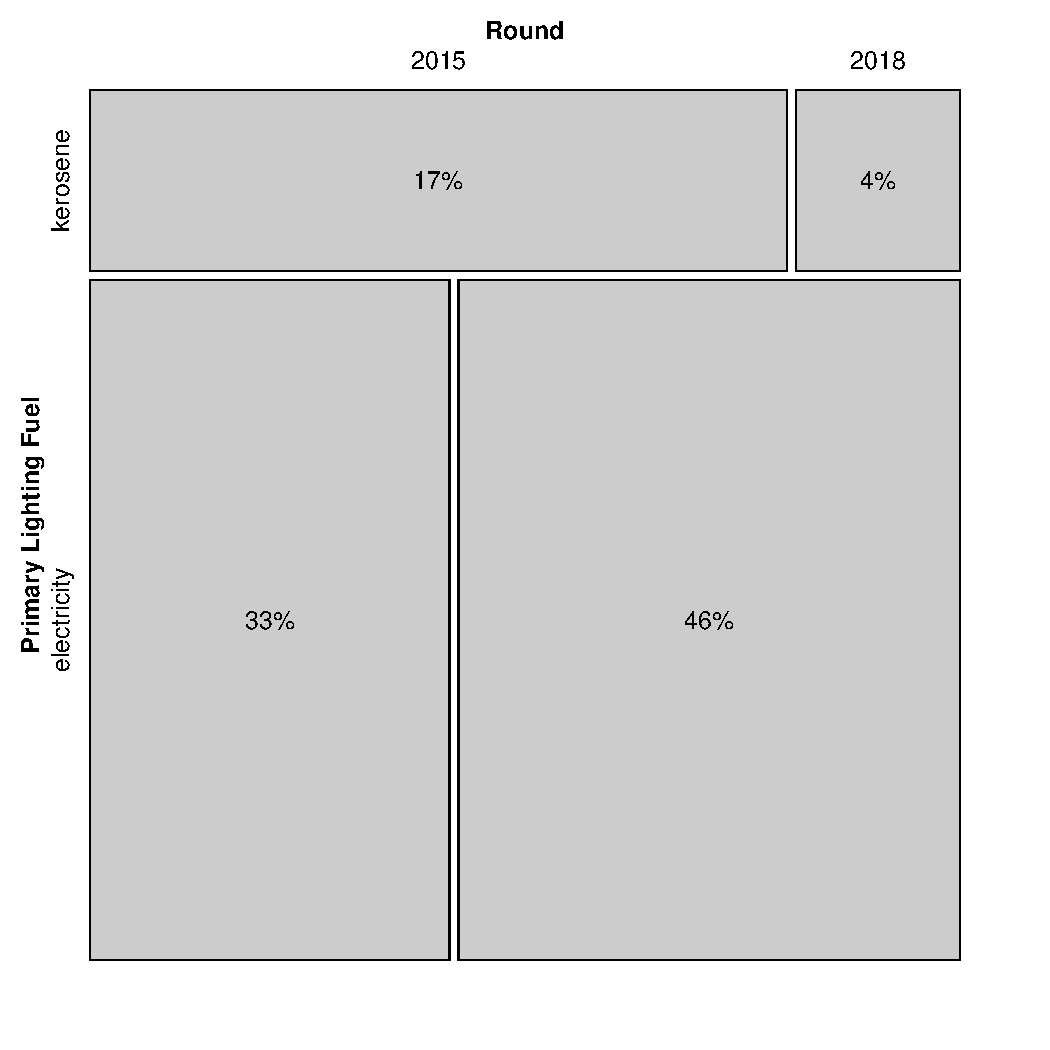
\includegraphics[scale=1]{Figures/Mosaic.pdf}
\caption{Mosaic plot of the proportion change in household primary lighting fuel choices. The figure shows the ratio difference of using electricity or kerosene as primary lighting fuel among our survey sample of 9,848 observations. The reported proportions are rounded to zero digits. The one-digit results are 17.1\%, 32.9\%, 4.5\%, 45.5\% accordingly.}
\label{mosaic}
\end{figure}

Our results also reveal that there is a discrepancy in lighting fuel choices between different states. Figure \ref{map} maps a state summary of the proportion of electrified households using kerosene as their primary lighting fuel in 2015 and 2018. Table \ref{states} shows the number of observations in each state and data on the change in kerosene share between 2015 and 2018. Among the six states, we find out that West Bengal has the lowest share of kerosene lamp usage in both rounds, followed by Odisha. Moreover, the differences between states decreased from 2015 to 2018. Tremendous improvement has been achieved in Jharkhand and Uttar Pradesh with a nearly 40 percentage points reduction in kerosene lamp primary users in 2018 compared to 2015. However, the changes in leading states such as West Bengal are not as significant, which reveals the stagnancy of transitioning to the modern lighting fuel among a certain portion of households.

\begin{figure*}
\centering
\begin{subfigure}[b]{\textwidth}
\centering
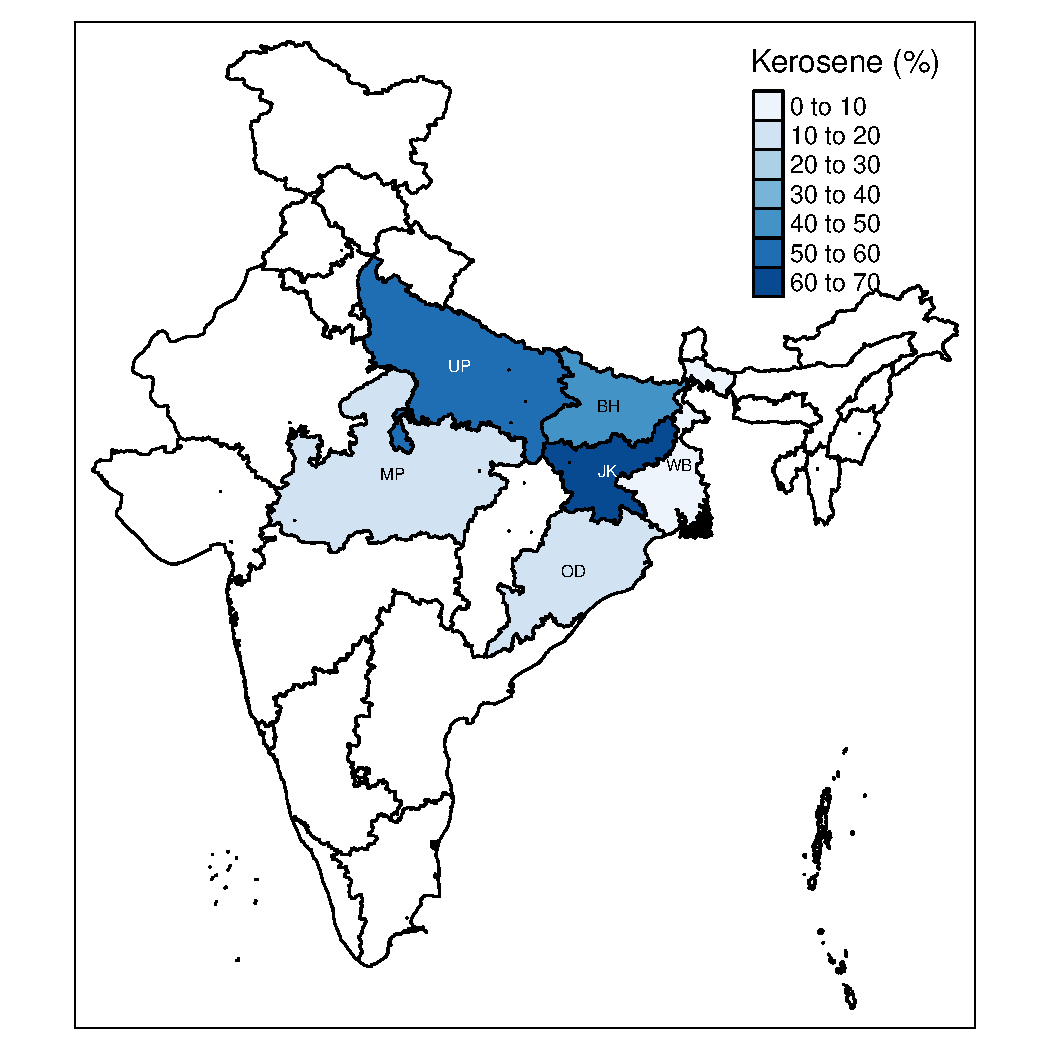
\includegraphics[width=0.5\textwidth]{Figures/Map_2015.pdf}
\caption{2015}
\end{subfigure}
\begin{subfigure}[b]{\textwidth}
\centering
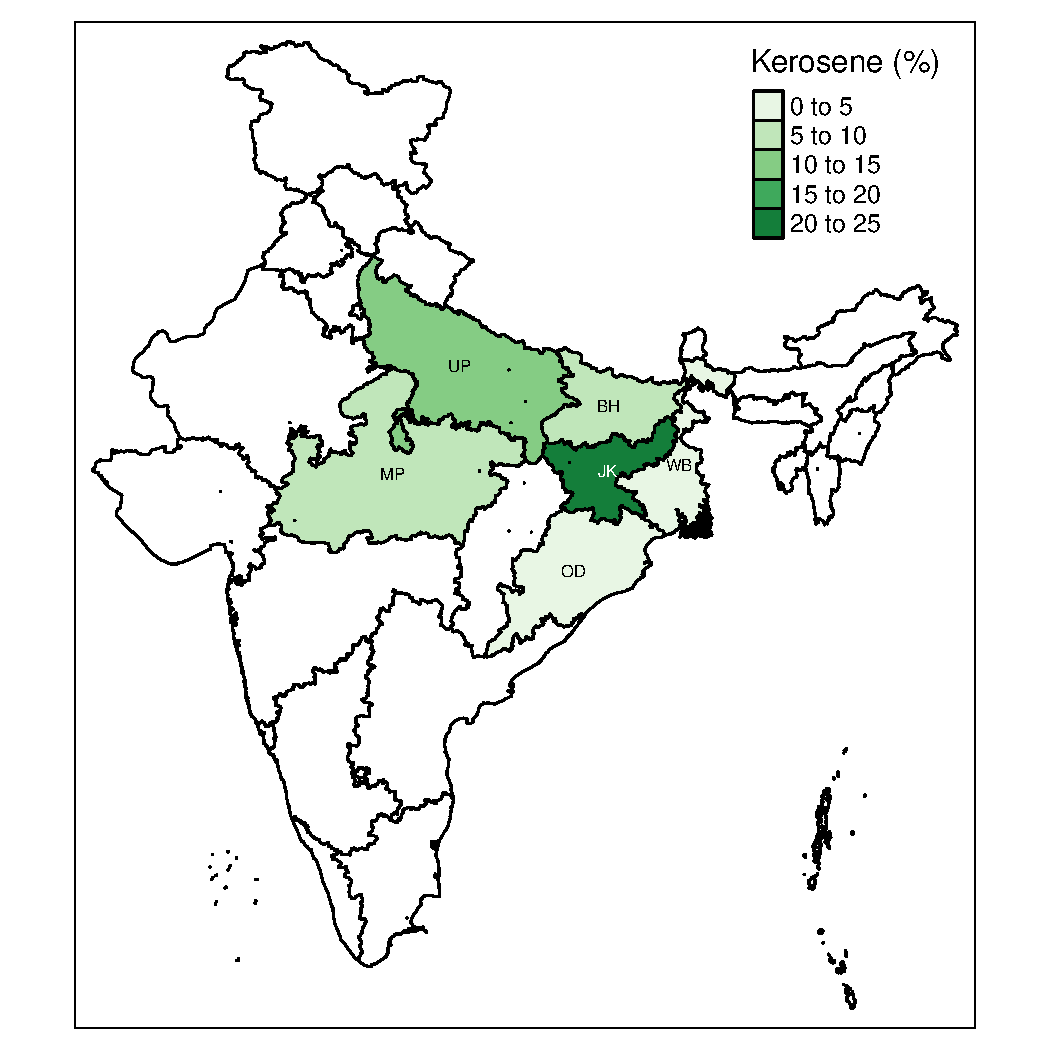
\includegraphics[width=0.5\textwidth]{Figures/Map_2018.pdf}
\caption{2018}
\end{subfigure}
\caption{Map of six surveyed states: Madhya Pradesh (MP), Uttar Pradesh (UP), Bihar (BH), Jharkhand (JK), Odisha (OD), and West Bengal (WB). The figure shows the adoption rate of kerosene as the primary lighting fuel in electrified households by state.}
\label{map}
\end{figure*}

\begin{table}[ht!]
\centering

% Table created by stargazer v.5.2.2 by Marek Hlavac, Harvard University. E-mail: hlavac at fas.harvard.edu
% Date and time: Mon, Apr 01, 2019 - 12:31:24 AM
\begin{tabular}{@{\extracolsep{5pt}} ccccc} 
\\[-1.8ex]\hline 
\hline \\[-1.8ex] 
 & State & N & 2015 Share of Kerosene (\%) & 2018 Share of Kerosene (\%) \\ 
\hline \\[-1.8ex] 
1 & Bihar & $588$ & $47$ & $8$ \\ 
2 & Jharkhand & $472$ & $66$ & $22$ \\ 
3 & Madhya Pradesh & $1,303$ & $16$ & $6$ \\ 
4 & Orissa & $181$ & $13$ & $1$ \\ 
5 & Uttar Pradesh & $1,468$ & $58$ & $14$ \\ 
6 & West Bengal & $912$ & $0$ & $0$ \\ 
\hline \\[-1.8ex] 
\end{tabular} 

\caption{Summary of sample numbers and change of share of kerosene in each of the six states}
\label{states}
\end{table}

\subsection{Explanatory Variables}

To analyze the relationship between electricity service quality and households$'$ primary lighting fuel choice, we use primary explanatory variables that represent the characteristics of electricity adequacy and reliability households experienced. These two aspects are the most basic characteristics of electricity supply quality, which largely dictate whether households will use electric lights for their illumination needs. Table \ref{sum_stats} summarizes the descriptive statistics with mean, standard deviation, minimum and maximum for the three explanatory variables we analyze. All the explanatory variables are in the form of numeric data.

For adequacy indicators, we use the responses in the survey data recorded for the question: $``$How many hours a day is electricity usually available?$"$ and $``$For how many hours is electricity usually available between sunset and midnight (till 12 o$'$clock)?$"$ To perform regression analysis, we create two variables: one for hours of available electricity during the night and the other for hours of available electricity during the daytime with the latter variable being calculated by deducting the result of the second question from the first question. Although this calculation will include service hours from midnight to early morning in daytime hours, this method is based on our assumption in the surveyed region that electricity is seldomly supplied during this period. The issue of electricity inadequacy commonly exists in the developing world and has been identified as a factor that largely influences people$'$s satisfaction of their electricity service \citep{DugouaUrpelainen2014, BakkerLachs2004}. We also identify the inadequacy problem as one of the most important issues in influencing Indian households$'$ choice of primary lighting fuel. Nighttime duration of electricity service is an important influencer as during this time lighting is at its peak demand. Due to the gap between high levels of usage and low supply during this time period, there is a high possibility that needs are not met. The data from Table \ref{sum_stats} shows that the availability of electricity during the night time is relatively short with an average of fewer than 4 hours.

In terms of electricity reliability, households experiencing electricity outage issues suffer from unsteady light and thus, express dissatisfaction \citep{Aklinetal2016}. We take the number of days without any electricity connection in a typical month as the predictor. We choose power outage over voltage fluctuations as an indicator because the latter is more closely related to the reliability of using larger appliances. Lighting lamps can be normally operated at a very low voltage. The question was designed as: $``$How many days in the last month has there been no power throughout the day?$"$. Power outages are important for electricity light use since, during the blackout days, no families can use electric lights and they must resort to using kerosene lamps. From Table \ref{sum_stats}, we see that there is a relatively high occurrence of the power outage days in India with an average of 3.8 days per month in 2015. And while the number of power outage days reduced to 2.1 days in 2018, it remains a crucial issue for Indian households.


\begin{table}[ht!]
\centering
\begin{subtable}[b]{\textwidth}
\centering

% Table created by stargazer v.5.2.2 by Marek Hlavac, Harvard University. E-mail: hlavac at fas.harvard.edu
% Date and time: Tue, Mar 10, 2020 - 10:54:42 PM
\begin{tabular}{@{\extracolsep{5pt}} cccccc} 
\\[-1.8ex]\hline 
\hline \\[-1.8ex] 
 & Mean & SD & Min & Max & Observations \\ 
\hline \\[-1.8ex] 
Primary Lighting Electricity & $0.658$ & $0.474$ & $0$ & $1$ & 4,924 \\ 
Electricity Hours (Night) & $3.320$ & $1.740$ & $0$ & $8$ & 4,924 \\ 
Electricity Hours (Day) & $9.450$ & $4.990$ & $0$ & $21$ & 4,924 \\ 
Electricity Outage & $3.760$ & $4.920$ & $0$ & $25$ & 4,924 \\ 
\hline \\[-1.8ex] 
\end{tabular} 

\caption{2015 Summary statistics for explanatory variables (mean, SD, min, max, count)}
\end{subtable}
\begin{subtable}[b]{\textwidth}
\centering

% Table created by stargazer v.5.2.2 by Marek Hlavac, Harvard University. E-mail: hlavac at fas.harvard.edu
% Date and time: Tue, Jun 18, 2019 - 9:51:50 PM
\begin{tabular}{@{\extracolsep{5pt}} cccccc} 
\\[-1.8ex]\hline 
\hline \\[-1.8ex] 
 & Mean & SD & Min & Max & Observations \\ 
\hline \\[-1.8ex] 
Primary Lighting Electricity & $0.910$ & $0.286$ & $0$ & $1$ & 4,924 \\ 
Electricity Hours (Night) & $3.830$ & $1.330$ & $0$ & $6$ & 4,924 \\ 
Electricity Hours (Day) & $11.800$ & $4.440$ & $0$ & $24$ & 4,924 \\ 
Electricity Outage & $2.070$ & $3.340$ & $0$ & $30$ & 4,924 \\ 
\hline \\[-1.8ex] 
\end{tabular} 

\caption{2018 Summary statistics for explanatory variables (mean, SD, min, max, count)}
\end{subtable}
\caption{Table shows the basic statistics of different explanatory variables including available hours of electricity service (night/day), outage days}
\label{sum_stats}
\end{table}

\subsection{Control Variables}

Besides the primary factors, we also include control variables in our model considerations. Our selection of covariates is mainly based on the literature review and reflects the common focus of previous research studies.


1) Household Expenditure: Due to the characteristics of survey design, we rely on the household monthly expenditure to represent household income. As an essential indicator of the economic situation of a household, monthly expenditure is associated with the number of appliances owned. It represents their capability to afford and their willingness to prioritize a more expensive modern lighting fuel. Previous research also indicates a correlation between a household$'$s income and their fuel choices \citep{Pachaurietal2004, Khandkeretal2012, Beheraetal2015}. In addition, studies also found that wealthier households are more likely to have better public services such as electricity \citep{Smitsetal2015}. Besides being a confounder in the model, household expenditure also serves as a pre-treatment. To make sure expenditure serves as a reliable indicator of household income, the survey question is elaborated as $``$How much is your expenditure on household needs in a typical month?$"$ Although electricity, in general, could bring wealth accumulation, we find weak evidence that the wealth level will have a systematic change when a household makes different lighting source choices \citep{PoncedeLeonBaridoetal2017}.

2) Education Level: How well the head of the household is educated also influences their decision in adopting cleaner lighting fuel. A higher level of education usually results in a better understanding and knowledge of the benefits of modern fuels and greater resolution to fully utilize the resource \citep{RaoReddy2007}. We utilize the responses for the question, $``$Level of education of the household head$"$ and simplify the answer at two levels. We use 1 for the education level of 10th standard or higher and 0 for otherwise, thus, setting the variable as a binary indicator.

3) Social Status: We use the survey roster record: $``$Government Caste Category$"$ as an indicator of a household$'$s social status. The options are set up as: 1 as $``$Scheduled Caste (SC)$"$, 2 as $``$Scheduled Tribe (ST)$"$, 3 as $``$Other Backward Class (OBC)$"$, 4 as $``$General$"$, 5 as $``$Others$"$, and 6 as $``$No Caste$"$. According to Saxena et al. (2018) \citep{Saxenaetal2018}, disadvantaged caste groups including Scheduled Castes and Muslims face inequalities in accessing electricity. They may find it more challenging to engage in the electricity provision process due to their perceived inferior social status. The Social status of an Indian household is one of the key cultural factors that could influence their decisions on energy use. We reclassify the choices by combining SC, ST, and OBC since they are government qualified disadvantaged people. In this way, we are using dummies where 1 stands as disadvantaged and 0 as not.


4) Gender Effects: We believe that the gender of the household decision-maker is another important indicator of the acceptance of modern lighting fuels. We use the survey question $``$Who in your household makes decisions on the purchase of durable goods?$"$ and record the results in four types: male head of household, female head of household, jointly and other. We assume that women decision-makers take a positive role in choosing modern lighting fuels since they spend more time using lighting to do the housework \citep{Rahutetal2016}. Women decision-makers are also disadvantaged in influencing the decision process of electricity provision quality \citep{Wintheretal2017}. We define the answer of the female head of household as 1 and others as 0.

5) Family Size: According to Pandey and Chaubal (2011) \citep{PandeyChaubal2011}, the family size negatively influences a household$'$s decision on clean fuel choice. This can be explained through the logic that more family members mean more demand for lighting and this high demand further leads to a higher possibility of electricity deficiency and preference to stack kerosene for lighting. We sum up the answers from $``$Number of adults living in this household permanently (as of now)$"$ and $``$Number of children living in this household permanently (as of now)$"$ as our family size variable.


6) Region Fixed Effect and Round Fixed Effect: We assume there are within-state and within-year variations on the dependent variable owing to regional economic differences in the states and inconsistent electricity system reforms through the years. Our analysis also supports our hypothesis that different states have considerable discrepancies in the proportion of households using kerosene as their primary lighting fuel. Meanwhile, we also observe a great difference between the two rounds. We believe that there should be different constants for each state and each round, and thus included these two fixed effects for the robustness of our models.

Table \ref{sum_stats_control} shows the descriptive statistics for all the control variables we use. For dummy caste and education variables, we summarize the statistics for each level.

\begin{table}[ht!]
\centering
\begin{subtable}[b]{\textwidth}
\centering

% Table created by stargazer v.5.2.2 by Marek Hlavac, Harvard University. E-mail: hlavac at fas.harvard.edu
% Date and time: Mon, Apr 01, 2019 - 12:47:47 AM
\begin{tabular}{@{\extracolsep{5pt}} cccccc} 
\\[-1.8ex]\hline 
\hline \\[-1.8ex] 
 & Mean & SD & Min & Max & Observations \\ 
\hline \\[-1.8ex] 
log (Monthly Expenditure) & $8.460$ & $0.599$ & $6.400$ & $11$ & 4,924 \\ 
Monthly Expenditure & $5,680$ & $4,150$ & $600$ & $60,000$ & 4,924 \\ 
Caste: SC/ST & $0.267$ & $$ & $0$ & $1$ & 4,924 \\ 
Caste: OBC & $0.458$ & $$ & $0$ & $1$ & 4,924 \\ 
Caste: General & $0.274$ & $$ & $0$ & $1$ & 4,924 \\ 
Male Household Head & $0.763$ & $$ & $0$ & $1$ & 4,924 \\ 
Family Size & $6.740$ & $3.610$ & $1$ & $46$ & 4,924 \\ 
Edu: No Formal Schooling & $0.266$ & $$ & $0$ & $1$ & 4,924 \\ 
Edu: Up To 5th Standard & $0.311$ & $$ & $0$ & $1$ & 4,924 \\ 
Edu: More Than 5th Standard & $0.423$ & $$ & $0$ & $1$ & 4,924 \\ 
\hline \\[-1.8ex] 
\end{tabular} 

\caption{2015 Summary statistics for control variables (mean, SD, min, max, count)}
\end{subtable}
\begin{subtable}[b]{\textwidth}
\centering

% Table created by stargazer v.5.2.2 by Marek Hlavac, Harvard University. E-mail: hlavac at fas.harvard.edu
% Date and time: Mon, Apr 01, 2019 - 12:48:02 AM
\begin{tabular}{@{\extracolsep{5pt}} cccccc} 
\\[-1.8ex]\hline 
\hline \\[-1.8ex] 
 & Mean & SD & Min & Max & Observations \\ 
\hline \\[-1.8ex] 
log (Monthly Expenditure) & $8.630$ & $0.627$ & $5.300$ & $11.300$ & 4,924 \\ 
Monthly Expenditure & $6,760$ & $4,750$ & $200$ & $80,000$ & 4,924 \\ 
Caste: SC/ST & $0.277$ & $$ & $0$ & $1$ & 4,924 \\ 
Caste: OBC & $0.455$ & $$ & $0$ & $1$ & 4,924 \\ 
Caste: General & $0.267$ & $$ & $0$ & $1$ & 4,924 \\ 
Male Household Head & $0.641$ & $$ & $0$ & $1$ & 4,924 \\ 
Family size & $6.240$ & $3.310$ & $1$ & $38$ & 4,924 \\ 
Edu: No Formal Schooling & $0.335$ & $$ & $0$ & $1$ & 4,924 \\ 
Edu: Up To 5th Standard & $0.316$ & $$ & $0$ & $1$ & 4,924 \\ 
Edu: More Than 5th Standard & $0.349$ & $$ & $0$ & $1$ & 4,924 \\ 
\hline \\[-1.8ex] 
\end{tabular} 

\caption{2018 Summary statistics for control variables (mean, SD, min, max, count)}
\end{subtable}
\caption{Table shows the basic statistics of different control variables including household expenditure, household social status, decision maker$’$s education level, decision maker$’$s gender, and household family size.}
\label{sum_stats_control}
\end{table}


\section{Results}

We summarize the satisfaction responses from the 4,924 electrified households in both rounds. We categorize the 4,924 households into four groups: using grid-electricity as the primary lighting source in both rounds, using kerosene as the primary lighting source in both rounds, switching from kerosene to electricity, and switching from electricity to kerosene.

Figure \ref{satisfaction1} shows households$'$ attitudes towards their primary fuels as satisfied, neutral, or unsatisfied in each group. People who used electricity as the primary lighting fuel in both rounds were more satisfied in 2018 (2,070 households) than in 2015 (1,596 households) (Figure \ref{satisfaction1}). This coincides with the improvement in electricity quality from 2015 to 2018 shown in Figure \ref{satisfaction2}. The figure shows that, in this group, the proportion of households that consider electricity services as inadequate, unreliable, unsafe, and expensive all declined. Households that switched from kerosene to electricity show a greater increase in satisfaction (from 244 households in 2015 to 737 households in 2018). This could be due to the improved adequacy and safety features of electricity services in 2018 (Figure \ref{satisfaction2}). However, Figure \ref{satisfaction2} shows a drastic increase in the number of households claiming to have unreliability issues after switching from kerosene to electricity. A considerable number of households that used electricity in 2018 reported electricity as unsatisfactory (397 households for un-switched electricity users and 349 households for kerosene-electricity switched users). Consistent with the previous findings, households that used electricity in 2015 and switched to kerosene in 2018 also found kerosene more reliable. Based on these results, we find that the reliability issue of electricity services was the key barrier for households to switch from kerosene to electricity; it was also possibly the primary driver for households to do the reverse switch.

\begin{figure}[h!]
\centering
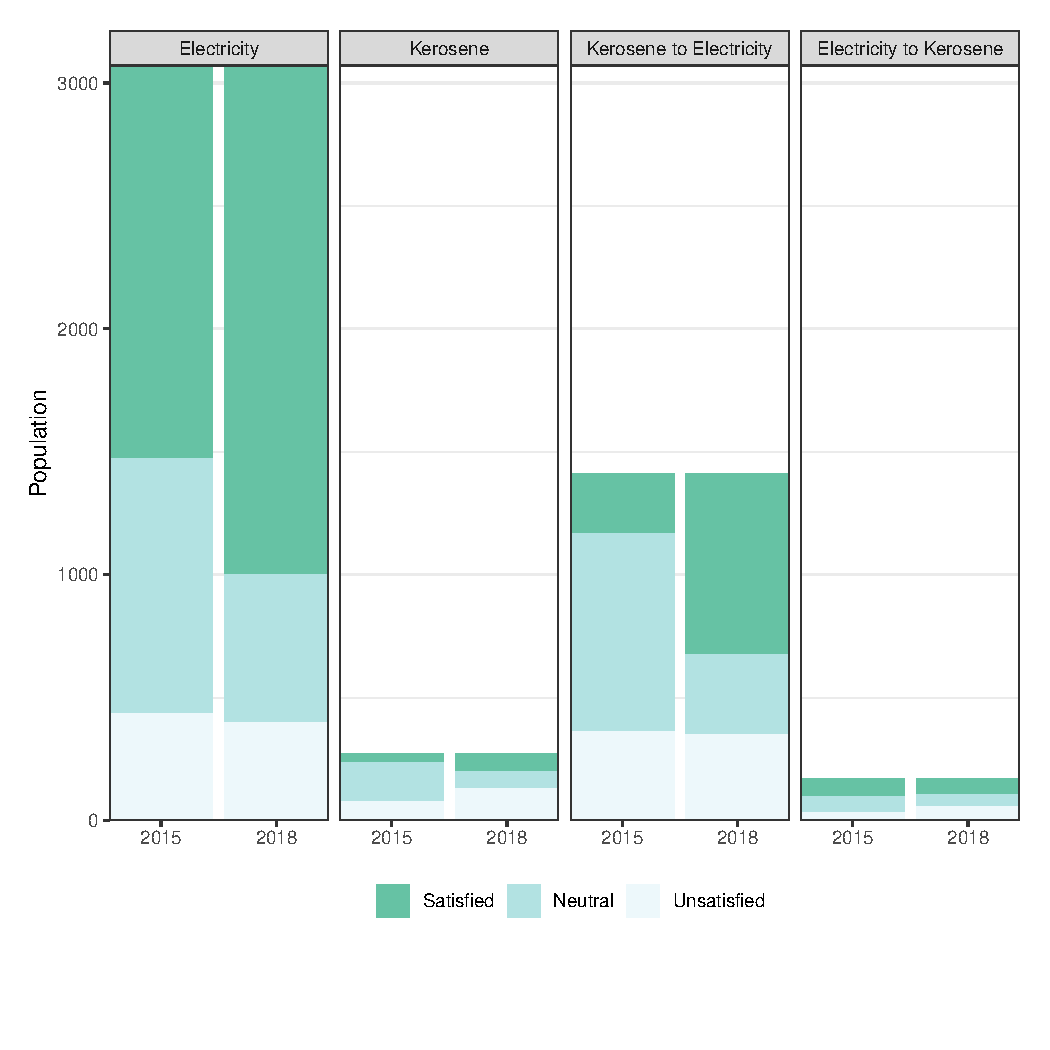
\includegraphics[scale=1]{Figures/Satisfaction1.pdf}
\caption{Stacked bar chart of household satisfaction levels from four groups in two rounds: using grid-electricity as the primary source of lighting fuel in both rounds, using kerosene as the primary source of lighting fuel in both rounds, switching from kerosene to electricity, and switching from electricity to kerosene. }
\label{satisfaction1}
\end{figure}

\begin{figure}[h!]
\centering
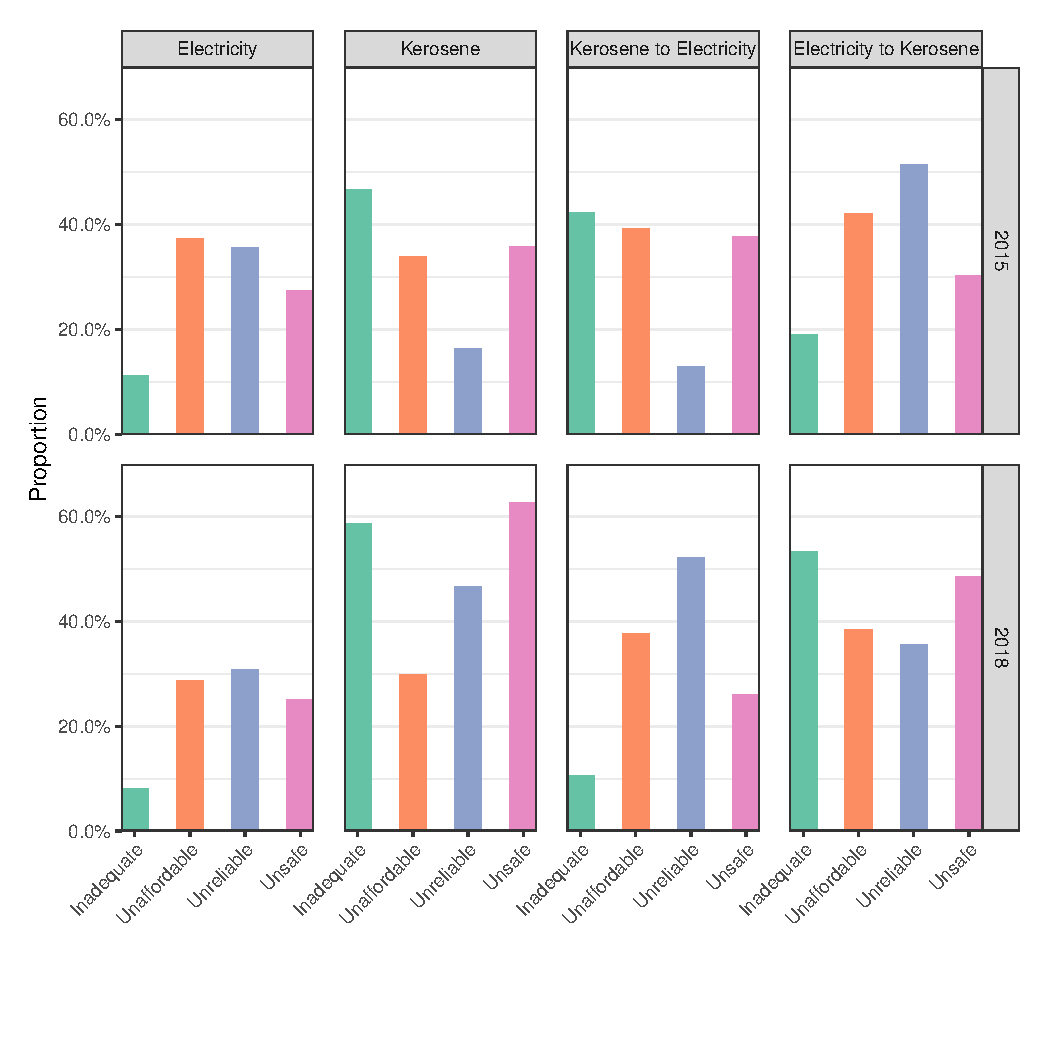
\includegraphics[scale=1]{Figures/Satisfaction2.pdf}
\caption{Figure shows households$'$ answers on the adequacy, affordability, reliability, and safety of the primary fuel they use in each round.}
\label{satisfaction2}
\end{figure}

For the logistic regression analysis, we test our model with and without control variables; we also test with and without the region and round fixed effects. We regress the dependent variable on different combinations of explanatory variables using six models in Table \ref{reg_results_explanatory}: We include daytime and nighttime duration of electricity service in model 1 and 2; we include fixed effects in model 2; model 3 and model 4 contain power outage days with or without fixed effects; and model 5 and model 6 include all three explanatory variables. The table shows our regression results with odds ratios and standard errors for each variable. Each coefficient represents the odds ratio of choosing electricity as primary lighting fuel over kerosene with one unit change in nighttime hours, daytime hours and blackout days, accordingly.

We calculate odds ratios from the original model coefficients by taking the exponential value of log-odds. In this case, an odds ratio larger than one means the predictor has a positive effect on the outcome, and an odds ratio smaller than one indicates that the increase in the independent variable will lead to a decrease in the dependent variable. By doing so, we are able to show the substantial influence of electricity duration and power outage days on the decision of whether to choose electricity as the primary lighting fuel. From the results, we show that adequacy and reliability of electricity supply are both closely related to households$'$ choices of primary lighting fuel. The households that report short duration hours and high frequency of outage days have a low probability of choosing electricity as their primary lighting fuel. Among the three factors we analyze, nighttime duration of electricity service has a larger influence on households$'$ decisions than daytime duration of electricity service. In detail, holding daytime service duration and outage days fixed, with an hour increase in nighttime electricity duration, we expect to see a 48\% increase in the odds of choosing electricity as primary lighting fuel. With one hour increase in day electricity duration, the odds of choosing electricity are expected to increase by 17\%. With one more power outage day, the odds of choosing electricity are expected to decrease by 3\%. We also notice that the odds ratios in the models with fixed effects are all closer to one, indicating that the issues of insufficient and unreliable electricity services become less important. The difference is relatively larger in nighttime electricity duration than in daytime service hours and in outage frequency. The results support our hypothesis that household primary lighting preference is highly correlated with daytime and nighttime electricity duration as well as frequency of outage days.

\begin{table}[ht!]
\centering
\resizebox{\columnwidth}{!}{%

\begin{tabular}{@{\extracolsep{5pt}}lcccccc} 
\\[-1.8ex]\hline 
\hline \\[-1.8ex] 
 & \multicolumn{6}{c}{\textit{Dependent variable:}} \\ 
\cline{2-7} 
\\[-1.8ex] & \multicolumn{6}{c}{Primary Lighting Fuel (1= Electricity, 0=Kerosene)} \\ 
\\[-1.8ex] & (1) & (2) & (3) & (4) & (5) & (6)\\ 
\hline \\[-1.8ex] 
 Electricity Hours (night) & 1.769$^{***}$ & 1.492$^{***}$ &  &  & 1.755$^{***}$ & 1.478$^{***}$ \\ 
  & (0.039) & (0.035) &  &  & (0.039) & (0.035) \\ 
  Electricity Hours (day) & 1.233$^{***}$ & 1.175$^{***}$ &  &  & 1.219$^{***}$ & 1.165$^{***}$ \\ 
  & (0.010) & (0.010) &  &  & (0.010) & (0.010) \\ 
  Electricity Outage &  &  & 0.886$^{***}$  & 0.927$^{***}$ & 0.961$^{***}$ & 0.971$^{***}$ \\ 
  &  &  & (0.005)  & (0.006) & (0.006) & (0.006) \\ 
 \hline \\[-1.8ex] 
Region FE? & No & Yes & No & Yes & No & Yes \\ 
Round FE? & No & Yes & No & Yes & No & Yes \\ 
Observations & 9,848 & 9,848 & 9,848 & 9,848 & 9,848 & 9,848 \\ 
\hline 
\hline \\[-1.8ex] 
\textit{Note:}  & \multicolumn{6}{r}{$^{*}$p$<$0.1; $^{**}$p$<$0.05; $^{***}$p$<$0.01} \\ 
\end{tabular} 

%
}
\caption{Odds ratios for different regression models with standard errors clustered by village}
\label{reg_results_explanatory}
\end{table}


Table \ref{reg_results_controls} shows models with control variables included. The settings for these six models are the same as in Table \ref{reg_results_explanatory}, except that control variables are included in all models. The odds ratios of explanatory variables don't change much in models with control variables, showing the robustness of the models. For the control variable of social caste class, we use general caste as a reference; for education level, we use no formal schooling as the reference level. From the p-value reported in Table \ref{reg_results_controls}, we can infer that the gender of the household head is not related to the adoption of electricity as the primary lighting fuel. Furthermore, the influence of gender can be both positive and negative in our models. These results reject the hypothesis of gender issue being a critical influence in households$'$ fuel decision-making process \citep{Rahutetal2016}. According to our results, larger families have lower adoption rates of electric lighting. The influence of education level is unclear. When including all covariates, the education level of more than 5th standard, compared to the level of no formal schooling, is positively related to the adoption of electricity as the primary lighting fuel; however, a household with up to 5th standard education is not significantly different from a household without any formal schooling. The differences are more obvious in models with both the region and round fixed effects included.



\begin{table}[ht!]
\centering
\resizebox{\columnwidth}{!}{%

\begin{tabular}{@{\extracolsep{5pt}}lcccccc} 
\\[-1.8ex]\hline 
\hline \\[-1.8ex] 
 & \multicolumn{6}{c}{\textit{Dependent variable:}} \\ 
\cline{2-7} 
\\[-1.8ex] & \multicolumn{6}{c}{Primary Lighting Fuel (1= Electricity, 0=Kerosene)} \\ 
\\[-1.8ex] & (1) & (2) & (3) & (4) & (5) & (6)\\ 
\hline \\[-1.8ex] 
  \textbf{Electricity Hours (night)} & 1.795$^{***}$ & 1.507$^{***}$ &  &  & 1.782$^{***}$ & 1.493$^{***}$ \\ 
  & (0.040) & (0.036) &  &  & (0.040) & (0.036) \\ 
  \textbf{Electricity Hours (day)} & 1.224$^{***}$ & 1.169$^{***}$ &  &  & 1.211$^{***}$ & 1.159$^{***}$ \\ 
  & (0.010) & (0.010) &  &  & (0.010) & (0.010) \\ 
   \textbf{Electricity Outage} &  &  & 0.891$^{***}$ & 0.928$^{***}$ & 0.962$^{***}$ & 0.970$^{***}$ \\ 
  &  &  & (0.005) & (0.006) & (0.006) & (0.006) \\ 
   \textbf{Monthly Expenditure (log)} & 1.682$^{***}$ & 1.612$^{***}$ & 1.737$^{***}$ & 1.691$^{***}$ & 1.668$^{***}$ & 1.612$^{***}$ \\ 
  & (0.087) & (0.090) & (0.078) & (0.088) & (0.086) & (0.090) \\ 
   \textbf{Caste:}  &  &  &  &  &  &  \\ 
  &  &  &  &  &  &  \\ 
  Caste (SC/ST) & 0.663$^{***}$ & 0.615$^{***}$ & 0.759$^{***}$ & 0.675$^{***}$ & 0.662$^{***}$ & 0.613$^{***}$ \\ 
  & (0.058) & (0.058) & (0.056) & (0.060) & (0.058) & (0.058) \\ 
  Caste (OBC) & 0.806$^{**}$ & 0.883 & 0.710$^{***}$ & 0.920 & 0.806$^{**}$ & 0.880 \\ 
  & (0.061) & (0.072) & (0.047) & (0.070) & (0.061) & (0.072) \\ 
   \textbf{Male Household Head} & 1.089 & 1.194$^{*}$ & 0.901 & 1.125 & 1.096 & 1.199$^{*}$ \\ 
  & (0.075) & (0.088) & (0.053) & (0.077) & (0.075) & (0.089) \\ 
   \textbf{Family Size} & 0.941$^{***}$ & 0.971$^{***}$ & 0.903$^{***}$ & 0.961$^{***}$ & 0.942$^{***}$ & 0.971$^{***}$ \\ 
  & (0.008) & (0.009) & (0.007) & (0.008) & (0.008) & (0.009) \\ 
  \textbf{Education:} &  &  &  &  &  &  \\ 
  &  &  &  &  &  &  \\ 
  Education (More than 5th Standard) & 1.042 & 1.443$^{***}$ & 0.943 & 1.529$^{***}$ & 1.048 & 1.444$^{***}$ \\ 
  & (0.078) & (0.115) & (0.061) & (0.114) & (0.078) & (0.116) \\ 
  Education (Up to 5th Standard) & 0.939 & 1.118 & 0.964 & 1.161$^{*}$ & 0.944 & 1.120 \\ 
  & (0.072) & (0.093) & (0.064) & (0.091) & (0.073) & (0.093) \\ 
  
 \hline \\[-1.8ex] 
Region FE? & No & Yes & No & Yes & No & Yes \\ 
Round FE? & No & Yes & No & Yes & No & Yes \\ 
Observations & 9,848 & 9,848 & 9,848 & 9,848 & 9,848 & 9,848 \\ 

\hline 
\hline \\[-1.8ex] 
\textit{Note:}  & \multicolumn{6}{r}{$^{*}$p$<$0.1; $^{**}$p$<$0.05; $^{***}$p$<$0.01} \\ 
\end{tabular} 

%
}
\caption{Odds ratios for different regression models with control variables included and standard errors clustered by village. The reference level for Caste is general caste; the reference level for Education is no formal schooling. }
\label{reg_results_controls}
\end{table}

Figure \ref{AME} shows the average marginal effects of our tested covariates on the probability of adopting electricity as the primary lighting option. We calculate the average marginal effect (AME) of each covariate from the full model (model (6) in Table \ref{reg_results_controls}). We use the average marginal effect (AME) instead of the marginal effect at the mean (MEM) to show the averaged effects among the analyzed households. On average, a one-hour increase in night electricity service increases the probability of adopting electricity as primary lighting fuel by 4.05 percentage points (95\% CI: 3.6-4.5 percentage points). Daytime service hour has a smaller substantial influence on the household choices of primary electric lights. One-hour increase in daytime service will lead to a 1.50 percentage points (95\% CI: 1.33-1.66 percentage points) increase in the probability of choosing electric lights as the primary. The number of outage days has a smaller impact than service hours. With one more outage day per month, households will have a 0.31 percentage points (95\% CI: 0.18-0.44 percentage points) lower probability, on average, for adopting electricity as their primary lighting option. It is also worth noticing that there is a potential collinearity issue between our explanatory variables of electricity supply. Households suffering from insufficient service hours are also likely to suffer from unreliable service, whereas households that have long service duration are generally in the regions with a better grid without many outages.

\begin{figure}[h!]
\centering
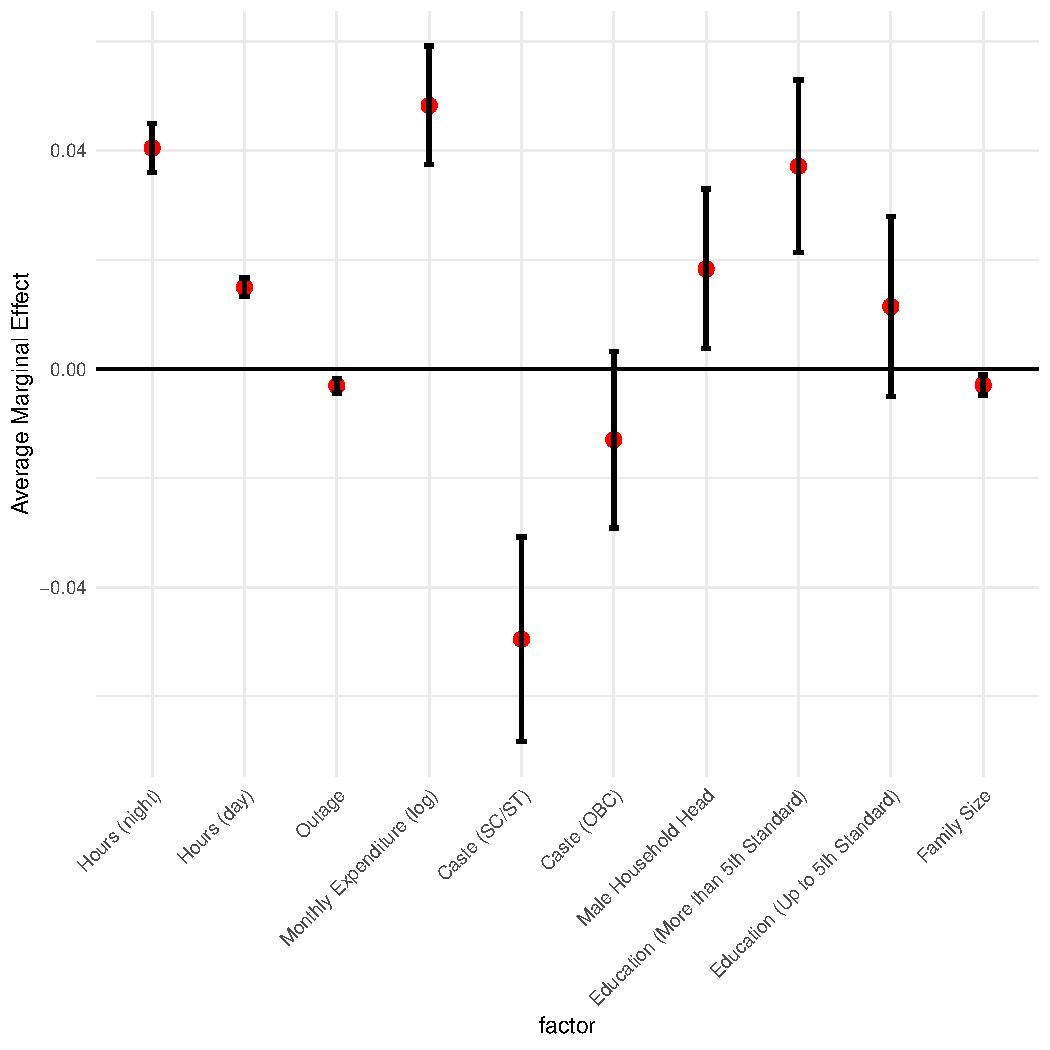
\includegraphics[scale=1]{Figures/AME.pdf}
\caption{The average marginal effects (AME) with confidence intervals of different variables analyzed in model (6) in Table \ref{reg_results_controls}. This figure presents the influence of each predictor on the probability of adopting electric lights as the primary choice. The red dots show the average changes in the probability of using electricity as primary lighting option when variables increase by 1 unit.}
\label{AME}
\end{figure}

\section{Conclusion and Policy Implications}

Electric lighting brings some of the primary benefits of modern electrification to the general public. The benefits include safety, efficiency, convenience, and public health. On the contrary, using traditional kerosene lamps results in serious health issues such as eye and respiratory diseases. The persistent reliance on kerosene among some members prevents the population from fully capturing the welfare of modern electrification. Using two-round panel data of six Indian states, we find that along with the continuous progress in electrification, a more effective scheme for improving the quality of electricity supply should be introduced as the next step to further promote modern lighting options.

Our analysis of household satisfaction on primary lighting fuel indicates that people who use electricity in 2018 were generally more satisfied with their fuel than in 2015. The population who recently transitioned to using electric lighting has the highest increase in satisfaction. To help households change their lighting use habits, improvements in the quality of electricity services are urgently needed. The results indicate the possibility that some households will return to using kerosene as their primary lighting fuel due to dissatisfaction with the electricity quality. To encourage them to use electricity, the reliability of electricity service needs to be improved significantly. The measure to increase the reliability of electricity would also benefit new electricity users since they also reported serious reliability issues with electricity supply in 2018.


Our results from the logistic regression suggest two core strategies that can be adopted by the government to help rural families transition from relying on kerosene lamps to using electric lights as their primary lighting choice. First, we identify that limited electricity supply duration, especially during peak hours, is discouraging households from using electric lights. We recommend that the government take concrete measures to ensure sufficient service during night peak hours. Second, we find that the high frequency of power outage provides motives for people to store and use kerosene lamps. To curb this, the government should implement policies to minimize power outages and maintain reliable and steady electricity supply. Only with a reliable supply can people see the benefits and convenience of using electric lights.

There are also opportunities for future research. Our sample of households that use electricity in both rounds may have caused a potential bias. Households that could have but decided not to obtain an electricity connection have self-selected out of the sample. Excluding this group will cause an overestimation of the electricity quality in our study. Being unsatisfied with electricity service, these households have a larger probability of poor electricity quality according to Aklin et al. (2016) \citep{Aklinetal2016}. Further studies that include more evidence from studies in other regions will enable the generalization of results and the development of common theory. In addition, the electrification rate has significantly increased since the first round of the survey, so the newly switched households - poorer, less educated - could behave differently. This leads to potential bias in our results. Meanwhile, to give more insight and analysis, policy-related variables in different states and rounds such as subsidy measures and level of concerns could be included. A cost-benefit analysis would be needed to give further recommendations on policy priorities. If more detailed data on lighting expenses could be collected, a more reliable outcome variable could be constructed with the quantitative records of fuel usage.

The study of household lighting fuel preferences depicts a broader picture of energy access in rural India. Considering the primary role of illumination in fulfilling households$'$ energy needs, understanding the reasons behind electrified household lighting preferences is essential for more progress with electrification. Our results show correlations between lighting fuel choices and electricity quality. We find that the poor quality of electricity service, including insufficient hours and frequent power outages, are major obstacles that deter households from transitioning to using cleaner fuel for lighting. Understanding the puzzle of the continued kerosene lighting fuel use is also informative for policymakers to infer reasons for other household energy choices. The government should further establish more profound schemes to improve electricity quality in order to achieve cleaner energy use and bring electricity benefits to a broader population.

\clearpage
%\setcitestyle{numbers}

\bibliographystyle{elsarticle-num}
\bibliography{PrimaryLightingFuel}
\end{document}
